%%%%%%%%%%%%%%%%%%%%%%%%%%%%%%%%%%%%%%%%%%%%%%
\section{Fossilized birth-death process}
%%%%%%%%%%%%%%%%%%%%%%%%%%%%%%%%%%%%%%%%%%%%%%

\begin{frame}{The problem}

\begin{itemize}

\item We have 
\begin{itemize}
  \item \normalsize{{\bf molecular data} of extant species,} 
  \item \normalsize{{\bf morphological data} of extant and fossil species and }
  \item \normalsize{{\bf Fossil ages} (or geological time intervals).}
\end{itemize} 
\item We want to utilise all this data to learn about {\bf evolutionary history} and {\bf macroevolutionary processes}.
\item {\bf Bayesian statistical inference} is our preferred method of learning about the world.


\end{itemize}

\end{frame}


%%%%%%%%%%%%%%%%%%%%%%%%%%%%%%%%%%%%%%%%%%%%%%


\begin{frame}{Node dating}

\begin{itemize}
\item {\bf Divergence time dating is tricky :) }
\item {\bf A common practice is node dating}. One or more divergences in a phylogeny are assigned ages by identifying fossils of known geological age that correspond* to each divergence. 
\item This method has a few drawbacks:
\begin{itemize}
\item Often only the oldest fossil in a calibrated clade is used,
\item Calibration densities are often {\it ad hoc},
\item Difficult* to combine calibrations with tree priors,
\item Computational complexity of some methods mean that only a few nodes can be calibrated (Heled \& Drummond 2012).
\end{itemize}
\end{itemize}

\end{frame}


%%%%%%%%%%%%%%%%%%%%%%%%%%%%%%%%%%%%%%%%%%%%%%


\begin{frame}{Tip dating and total evidence}

Two main features of new method for divergence-time dating:
\begin{itemize}
\item Explicit modelling of fossilization events as a part of the tree branching process (Pyron 2011, Heath {\it et al} 2014),
\item Utilising all existing data \textcolor{newblue1}{(total evidence)} in a joint inference (Pyron 2011, Ronquist {\it et al} 2012).
\end{itemize}

\end{frame}


%%%%%%%%%%%%%%%%%%%%%%%%%%%%%%%%%%%%%%%%%%%%%%


%\begin{frame}{Total evidence}

%\begin{itemize}

%\item Pyron 2011 uses Lewis MK model to model evolution of morphological characters.  
%\item Ronquist et al 2012, Wood et al 2012. 
%\item They used Yule or Uniform tree prior. 
%\end{itemize}


%\end{frame}
 

%%%%%%%%%%%%%%%%%%%%%%%%%%%%%%%%%%%%%%%%%%%%%%


\begin{frame}{Birth-death-sampling models}

\begin{figure}
  \begin{center}
               \usetikzlibrary{shapes,snakes}

\begin{tikzpicture}[thick, scale=0.6, color=gray]

\begin{scope}

%terminal nodes
\node at (-3.5, 2.5)(s2){};
\node at (0, 1)(s3){};
\node at (-2.5, 1)(s4){};
\node at (4, 3.1)(s5){};
\node at (1.4, 3.5)(s7){};
\node at (-1, 1)(s8){};
\node at (3.2, 1)(s9){};
\node at (2, 1)(s10){};

%branches
\draw (0, 7.5) -- (0,7) -- (-2, 7) --(-2, 5.5) --(-3, 5.5) -- (-3, 4.9) -- (-3.5, 4.9) -- (s2);
\draw (-3, 4.9) -- (-2.5, 4.9) -- (s4); 
\draw (-2, 5.5) -- (-1, 5.5) -- (s8); 
\draw (0,7) -- (2,7) -- (2,5.8) -- (0.7, 5.8) -- (0.7, 4.5) -- (0, 4.5) -- (s3); 
\draw (0.7, 4.5) -- (1.4, 4.5) -- (s7); 
\draw (2, 5.8) -- (3.3, 5.8) -- (3.3, 4) -- (2.6, 4) -- (2.6, 2.1) -- (2, 2.1) -- (s10); 
\draw (2.6, 2.1) -- (3.2, 2.1) -- (s9);
\draw (3.3, 4) -- (4, 4) -- (s5);

\node at (0, -1) {Full tree};

\pause 

%sampled nodes
\node[fill,circle, inner sep=2pt] at (-2.5, 1)(sA){};
\node[anchor=north] (Alet) at (sA) {\textcolor{black}{\footnotesize A}};
\node[fill,circle, inner sep=2pt] at (0, 1)(sB){};
\node[anchor=north] (Alet) at (sB) {\textcolor{black}{\footnotesize B}};
\node[fill,circle, inner sep=2pt] at (2, 1)(sC){};
\node[anchor=north] (Alet) at (sC) {\textcolor{black}{\footnotesize C}};
\node[fill,circle, inner sep=2pt] at (3.2, 1)(sD){};
\node[anchor=north] (Alet) at (sD) {\textcolor{black}{\footnotesize D}};

\pause 

\node[fill,circle, inner sep=2pt] at (3.3, 5)(sE){};
\node[anchor=west] (Alet) at (sE) {\textcolor{black}{\footnotesize E}};
\node[fill,circle, inner sep=2pt] at (-1, 2.9)(sF){};
\node[anchor=west] (Alet) at (sF) {\textcolor{black}{\footnotesize F}};

\pause 

\color{newblue1}

%branches
\draw (0, 7.5) -- (0,7) -- (-2, 7) --(-2, 5.5) --(-3, 5.5) -- (-3, 4.9);
\draw (-3, 4.9) -- (-2.5, 4.9) -- (s4); 
\draw (-2, 5.5) -- (-1, 5.5) -- (sF); 
\draw (0,7) -- (2,7) -- (2,5.8) -- (0.7, 5.8) -- (0.7, 4.5) -- (0, 4.5) -- (s3); 
\draw (2, 5.8) -- (3.3, 5.8) -- (3.3, 4) -- (2.6, 4) -- (2.6, 2.1) -- (2, 2.1) -- (s10); 
\draw (2.6, 2.1) -- (3.2, 2.1) -- (s9);

%sampled nodes
\node[fill,circle, inner sep=2pt] at (-2.5, 1)(sA){};
\node[anchor=north] (Alet) at (sA) {\textcolor{black}{\footnotesize A}};
\node[fill,circle, inner sep=2pt] at (0, 1)(sB){};
\node[anchor=north] (Alet) at (sB) {\textcolor{black}{\footnotesize B}};
\node[fill,circle, inner sep=2pt] at (2, 1)(sC){};
\node[anchor=north] (Alet) at (sC) {\textcolor{black}{\footnotesize C}};
\node[fill,circle, inner sep=2pt] at (3.2, 1)(sD){};
\node[anchor=north] (Alet) at (sD) {\textcolor{black}{\footnotesize D}};

\node[fill,circle, inner sep=2pt] at (3.3, 5)(sE){};
\node[anchor=west] (Alet) at (sE) {\textcolor{black}{\footnotesize E}};
\node[fill,circle, inner sep=2pt] at (-1, 2.9)(sF){};
\node[anchor=west] (Alet) at (sF) {\textcolor{black}{\footnotesize F}};

\end{scope}

\begin{scope}[xshift=8.5cm]

\color{white}

%terminal nodes
\node[fill,circle, inner sep=2pt] at (-3, 1)(sA){};
\node[anchor=north] (Alet) at (sA) {\textcolor{white}{\footnotesize A}};
\node[fill,circle, inner sep=2pt] at (0.7, 1)(sB){};
\node[anchor=north] (Alet) at (sB) {\textcolor{white}{\footnotesize B}};
\node[fill,circle, inner sep=2pt] at (2.7, 1)(sC){};
\node[anchor=north] (Alet) at (sC) {\textcolor{white}{\footnotesize C}};
\node[fill,circle, inner sep=2pt] at (3.9, 1)(sD){};
\node[anchor=north] (Alet) at (sD) {\textcolor{white}{\footnotesize D}};
\node[fill,circle, inner sep=2pt] at (-1, 2.9)(sF){};
\node[anchor=west] (Alet) at (sF) {\textcolor{white}{\footnotesize F}};
\node[fill,circle, inner sep=2pt] at (3.3, 5)(sE){};
\node[anchor=west] (Alet) at (sE) {\textcolor{white}{\footnotesize E}};

%branches
\draw (0, 7.5) -- (0,7) -- (-2, 7) --(-2, 5.5) --(-3, 5.5)  -- (sA);
\draw (-2, 5.5) -- (-1, 5.5) -- (sF); 
\draw (0,7) -- (2,7) -- (2,5.8) -- (0.7, 5.8) -- (0.7, 4.5) -- (sB); 
\draw (2, 5.8) -- (3.3, 5.8) -- (3.3, 4) -- (3.3, 2.1) -- (2.7, 2.1) -- (sC); 
\draw (3.3, 2.1) -- (3.9, 2.1) -- (sD);

\end{scope}

\end{tikzpicture}


            \end{center}
            
         \end{figure}    
\end{frame}


%%%%%%%%%%%%%%%%%%%%%%%%%%%%%%%%%%%%%%%%%%%%%% 


\begin{frame}{Birth-death-sampling models}


 \begin{figure}
            \begin{center}
               \usetikzlibrary{shapes,snakes}

\begin{tikzpicture}[thick, scale=0.6, color=gray]

\begin{scope}

%terminal nodes
\node at (-3.5, 2.5)(s2){};
\node at (0, 1)(s3){};
\node at (-2.5, 1)(s4){};
\node at (4, 3.1)(s5){};
\node at (1.4, 3.5)(s7){};
\node at (-1, 1)(s8){};
\node at (3.2, 1)(s9){};
\node at (2, 1)(s10){};

%branches
\draw (0, 7.5) -- (0,7) -- (-2, 7) --(-2, 5.5) --(-3, 5.5) -- (-3, 4.9) -- (-3.5, 4.9) -- (s2);
\draw (-3, 4.9) -- (-2.5, 4.9) -- (s4); 
\draw (-2, 5.5) -- (-1, 5.5) -- (s8); 
\draw (0,7) -- (2,7) -- (2,5.8) -- (0.7, 5.8) -- (0.7, 4.5) -- (0, 4.5) -- (s3); 
\draw (0.7, 4.5) -- (1.4, 4.5) -- (s7); 
\draw (2, 5.8) -- (3.3, 5.8) -- (3.3, 4) -- (2.6, 4) -- (2.6, 2.1) -- (2, 2.1) -- (s10); 
\draw (2.6, 2.1) -- (3.2, 2.1) -- (s9);
\draw (3.3, 4) -- (4, 4) -- (s5);

\node at (0, -1) {Full tree};

%sampled nodes
\node[fill,circle, inner sep=2pt] at (-2.5, 1)(sA){};
\node[anchor=north] (Alet) at (sA) {\textcolor{black}{\footnotesize A}};
\node[fill,circle, inner sep=2pt] at (0, 1)(sB){};
\node[anchor=north] (Alet) at (sB) {\textcolor{black}{\footnotesize B}};
\node[fill,circle, inner sep=2pt] at (2, 1)(sC){};
\node[anchor=north] (Alet) at (sC) {\textcolor{black}{\footnotesize C}};
\node[fill,circle, inner sep=2pt] at (3.2, 1)(sD){};
\node[anchor=north] (Alet) at (sD) {\textcolor{black}{\footnotesize D}};
\node[fill,circle, inner sep=2pt] at (3.3, 5)(sE){};
\node[anchor=west] (Alet) at (sE) {\textcolor{black}{\footnotesize E}};
\node[fill,circle, inner sep=2pt] at (-1, 2.9)(sF){};
\node[anchor=west] (Alet) at (sF) {\textcolor{black}{\footnotesize F}};


\color{newblue1}

%branches
\draw (0, 7.5) -- (0,7) -- (-2, 7) --(-2, 5.5) --(-3, 5.5) -- (-3, 4.9);
\draw (-3, 4.9) -- (-2.5, 4.9) -- (s4); 
\draw (-2, 5.5) -- (-1, 5.5) -- (sF); 
\draw (0,7) -- (2,7) -- (2,5.8) -- (0.7, 5.8) -- (0.7, 4.5) -- (0, 4.5) -- (s3); 
\draw (2, 5.8) -- (3.3, 5.8) -- (3.3, 4) -- (2.6, 4) -- (2.6, 2.1) -- (2, 2.1) -- (s10); 
\draw (2.6, 2.1) -- (3.2, 2.1) -- (s9);

%sampled nodes
\node[fill,circle, inner sep=2pt] at (-2.5, 1)(sA){};
\node[anchor=north] (Alet) at (sA) {\textcolor{black}{\footnotesize A}};
\node[fill,circle, inner sep=2pt] at (0, 1)(sB){};
\node[anchor=north] (Alet) at (sB) {\textcolor{black}{\footnotesize B}};
\node[fill,circle, inner sep=2pt] at (2, 1)(sC){};
\node[anchor=north] (Alet) at (sC) {\textcolor{black}{\footnotesize C}};
\node[fill,circle, inner sep=2pt] at (3.2, 1)(sD){};
\node[anchor=north] (Alet) at (sD) {\textcolor{black}{\footnotesize D}};
\node[fill,circle, inner sep=2pt] at (3.3, 5)(sE){};
\node[anchor=west] (Alet) at (sE) {\textcolor{black}{\footnotesize E}};
\node[fill,circle, inner sep=2pt] at (-1, 2.9)(sF){};
\node[anchor=west] (Alet) at (sF) {\textcolor{black}{\footnotesize F}};


\end{scope}

\begin{scope}[xshift=8.5cm]

\color{newblue1}

%terminal nodes
\node[fill,circle, inner sep=2pt] at (-3, 1)(sA){};
\node[anchor=north] (Alet) at (sA) {\textcolor{black}{\footnotesize A}};
\node[fill,circle, inner sep=2pt] at (0.7, 1)(sB){};
\node[anchor=north] (Alet) at (sB) {\textcolor{black}{\footnotesize B}};
\node[fill,circle, inner sep=2pt] at (2.7, 1)(sC){};
\node[anchor=north] (Alet) at (sC) {\textcolor{black}{\footnotesize C}};
\node[fill,circle, inner sep=2pt] at (3.9, 1)(sD){};
\node[anchor=north] (Alet) at (sD) {\textcolor{black}{\footnotesize D}};
\node[fill,circle, inner sep=2pt] at (-1, 2.9)(sF){};
\node[anchor=west] (Alet) at (sF) {\textcolor{black}{\footnotesize F}};
\node[fill,circle, inner sep=2pt] at (3.3, 5)(sE){};
\node[anchor=west] (Alet) at (sE) {\textcolor{black}{\footnotesize E}};

%branches

\draw (0, 7.5) -- (0,7) -- (-2, 7) --(-2, 5.5) --(-3, 5.5)  -- (sA);
\draw (-2, 5.5) -- (-1, 5.5) -- (sF); 
\draw (0,7) -- (2,7) -- (2,5.8) -- (0.7, 5.8) -- (0.7, 4.5) -- (sB); 
\draw (2, 5.8) -- (3.3, 5.8) -- (3.3, 4) -- (3.3, 2.1) -- (2.7, 2.1) -- (sC); 
\draw (3.3, 2.1) -- (3.9, 2.1) -- (sD);

\node at (0.6, -1) {\textcolor{newblue1}{Sampled tree}};

\end{scope}

\end{tikzpicture}


            \end{center}
            
         \end{figure}
    
\end{frame}


%%%%%%%%%%%%%%%%%%%%%%%%%%%%%%%%%%%%%%%%%%%%%% 


\begin{frame} {Fossillized birth-death model (FBD)}


\begin{columns}[t]
\begin{column}{.5\textwidth}

Stadler 2010, Heath {\it et al} 2014. 
\vspace{0.2cm}

The process starts at time $t_{or}>0$ and ends at time zero (present time).  
  \vspace{0.01cm}
   \begin{itemize}
\item birth rate $\lambda$
\item death rate $\mu$
\item sampling rate $\psi$
\item sampling at present probability $\rho$ 
   \end{itemize}
\vspace{0.01cm}

   \end{column}
   \begin{column}{.5\textwidth}

            \begin{center}
               \usetikzlibrary{shapes,snakes}

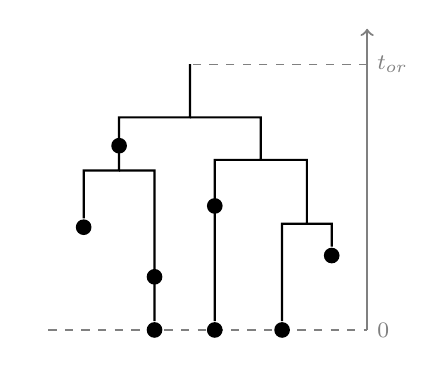
\begin{tikzpicture}[thick,scale=0.45]

\begin{scope}

\draw[ -> ,color=gray] (5, 1) -- (5, 9.5);
\draw[thin,dashed,color=gray] (5, 8.5) -- (0, 8.5);

\node[anchor=west]  at (5, 8.5) (or) {\textcolor{gray}{\footnotesize $t_{or}$}};

\draw[thin,dashed, color=gray] (-4, 1) -- (5, 1);
\node[anchor=west]  at (5, 1) (zero) {\textcolor{gray}{\footnotesize $0$}};



%sampled nodes
\node[fill,circle, inner sep=2pt] at (-3, 3.9)(s2){};
\node[fill,circle, inner sep=2pt] at (0.7, 4.5)(s1){};
\node[fill,circle, inner sep=2pt] at (0.7, 1)(s3){};
\node[fill,circle, inner sep=2pt] at (-2, 6.2)(s4){};
\node[fill,circle, inner sep=2pt] at (4, 3.1)(s5){};
\node[fill,circle, inner sep=2pt] at (-1, 1)(s8){};
\node[fill,circle, inner sep=2pt] at (-1, 2.5)(s9){};
\node[fill,circle, inner sep=2pt] at (2.6, 1)(s10){};


%branches
\draw (0, 8.5) -- (0,7) -- (-2, 7) --(-2, 5.5) --(-3, 5.5) -- (-3, 4.9) -- (s2);
\draw (-2, 5.5) -- (-1, 5.5) -- (s8); 
\draw (0,7) -- (2,7) -- (2,5.8) -- (0.7, 5.8) -- (0.7, 4.5) -- (s3); 
\draw (2, 5.8) -- (3.3, 5.8) -- (3.3, 4) -- (2.6, 4) --  (s10); 
\draw (3.3, 4) -- (4, 4) -- (s5);



\end{scope}



\end{tikzpicture}




            \end{center}
         
         \begin{center}\emph{Sampled tree} \end{center}   

   \end{column}    
\end{columns}

\vspace{0.2cm}

Model parameters: \color{newblue1} $\eta = (t_{or}, \lambda, \mu, \psi, \rho)$.

\color{black}
All the parameters are identifiable. 

\vspace{1.5cm}


\end{frame}


%%%%%%%%%%%%%%%%%%%%%%%%%%%%%%%%%%%%%%%%%%%%%%


\begin{frame} {Fossilized birth-death (FBD) skyline model}

Stadler \& K\"uhnert et al 2012, Gavryushkina {\it et al} 2014.

\vspace{0.2cm}

There are $k$ time intervals and parameters remain constants within the intervals but may vary from one interval to another

\begin{columns}[c]
\begin{column}{.5\textwidth}
\begin{itemize}
\item birth rates $\lambda_1, \ldots, \lambda_k$
\item death rates $\mu_1, \ldots, \mu_k$
\item sampling rates $\psi_1, \ldots, \psi_k$
\item sampling at time $t_k$ (present) probability $\rho$
\end{itemize}

\begin{center}
Model parameters:
\color{newblue1} $\eta = (t_{or}, \bar \lambda, \bar \mu, \bar \psi, \rho)$ 

\end{center}
  \end{column}
   \begin{column}{.5\textwidth}
\begin{center}
\usetikzlibrary{shapes,snakes}

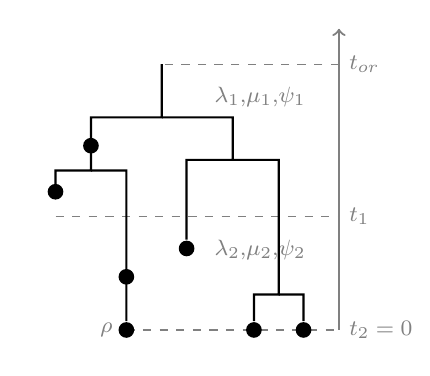
\begin{tikzpicture}[thick,scale=0.45]

\begin{scope}

\draw[ -> ,color=gray] (5, 1) -- (5, 9.5);
\draw[thin,dashed,color=gray] (5, 8.5) -- (0, 8.5);
\node[anchor=west]  at (5, 8.5) (or) {\textcolor{gray}{\footnotesize $t_{or}$}};

\draw[thin,dashed,color=gray] (-3, 4.2) -- (5, 4.2);
\node[anchor=west]  at (5, 4.2) (t1) {\textcolor{gray}{\footnotesize $t_1$}};


\draw[thin, dashed,color=gray] (-1, 1) -- (5, 1);
\node[anchor=west]  at (5, 1) (zero) {\textcolor{gray}{\footnotesize $t_2=0$}};

\node[anchor=south west]  at (1.2, 7.0) (y) {\textcolor{gray}{\footnotesize $\lambda_1$,$\mu_1$,$\psi_1$}};

\node[anchor=south west]  at (1.2, 2.7) (y) {\textcolor{gray}{\footnotesize $\lambda_2$,$\mu_2$,$\psi_2$}};

%\node[anchor=east]  at (-3.1, 4.2) (y) {\textcolor{gray}{\footnotesize $\rho_1$}};
\node[anchor=east]  at (-1.1, 1) (y) {\textcolor{gray}{\footnotesize $\rho$}};




%sampled nodes
\node[fill,circle, inner sep=2pt] at (-3, 4.9)(s2){};
\node[fill,circle, inner sep=2pt] at (0.7, 3.3)(s3){};
\node[fill,circle, inner sep=2pt] at (-2, 6.2)(s4){};
\node[fill,circle, inner sep=2pt] at (4, 1)(s5){};
\node[fill,circle, inner sep=2pt] at (-1, 1)(s8){};
\node[fill,circle, inner sep=2pt] at (-1, 2.5)(s9){};
\node[fill,circle, inner sep=2pt] at (2.6, 1)(s10){};


%branches
\draw (0, 8.5) -- (0,7) -- (-2, 7) --(-2, 5.5) --(-3, 5.5) -- (-3, 4.9) -- (s2);
\draw (-2, 5.5) -- (-1, 5.5) -- (s8); 
\draw (0,7) -- (2,7) -- (2,5.8) -- (0.7, 5.8) -- (0.7, 4.5) -- (s3); 
\draw (2, 5.8) -- (3.3, 5.8) -- (3.3, 2) -- (2.6, 2) --  (s10); 
\draw (3.3, 2) -- (4, 2) -- (s5);

\end{scope}



\end{tikzpicture}


\end{center}
\begin{center}\emph{\small Sampled tree} \end{center}   
 \end{column}    
\end{columns}

\end{frame}


%%%%%%%%%%%%%%%%%%%%%%%%%%%%%%%%%%%%%%%%%%%%%%

\iffalse 

\begin{frame}{Variation in the choice of the tree model parameters}

The $t_{or}$ parameter can be replaced with $t_{root}$ parameter assuming the process started with a branching event. 

\vskip2mm

Instead of $\lambda$, $\mu$, and $\psi$ we can also use an alternative parameterisation:

\renewcommand{\arraystretch}{1.2}

\begin{equation*} 
\begin{tabular}{ll} 
\text{net diversification rate} & $d = \lambda-\mu$  \\ 
\text{turnover rate} & $\turnover = \frac \mu \lambda$ \\ 
\text{\sampleprop} & $\fosp = \frac\psi {\mu + \psi}$  \\ 
\end{tabular} \end{equation*}

\end{frame}

\fi
%%%%%%%%%%%%%%%%%%%%%%%%%%%%%%%%%%%%%%%%%%%%%%


\begin{frame}{Heath {\it et al} approach and its extensions}

 Heath {\it et al} 2014 first used FBD model to infer divergence times of bears in a Bayesian MCMC framework:  

\begin{itemize}
\item The topology of extant species is fixed
\item Only used occurrence dates of fossils, and no morphology 
\item Fixed $\rho$ to the truth in the inference
\end{itemize}

We extend this model in two ways:

\begin{itemize}
\item Sampling sampled ancestor trees (Gavryushkina {\it et al} 2014)
\item Incorparating morphological data
\end{itemize}

Implemented in SA and Morph-models packages for BEAST2 (\url{www.beast2.org})

\end{frame}


%%%%%%%%%%%%%%%%%%%%%%%%%%%%%%%%%%%%%%%%%%%%%%


\begin{frame}{Comparative data of fossil tips vs only occurrence dates}

\begin{figure}
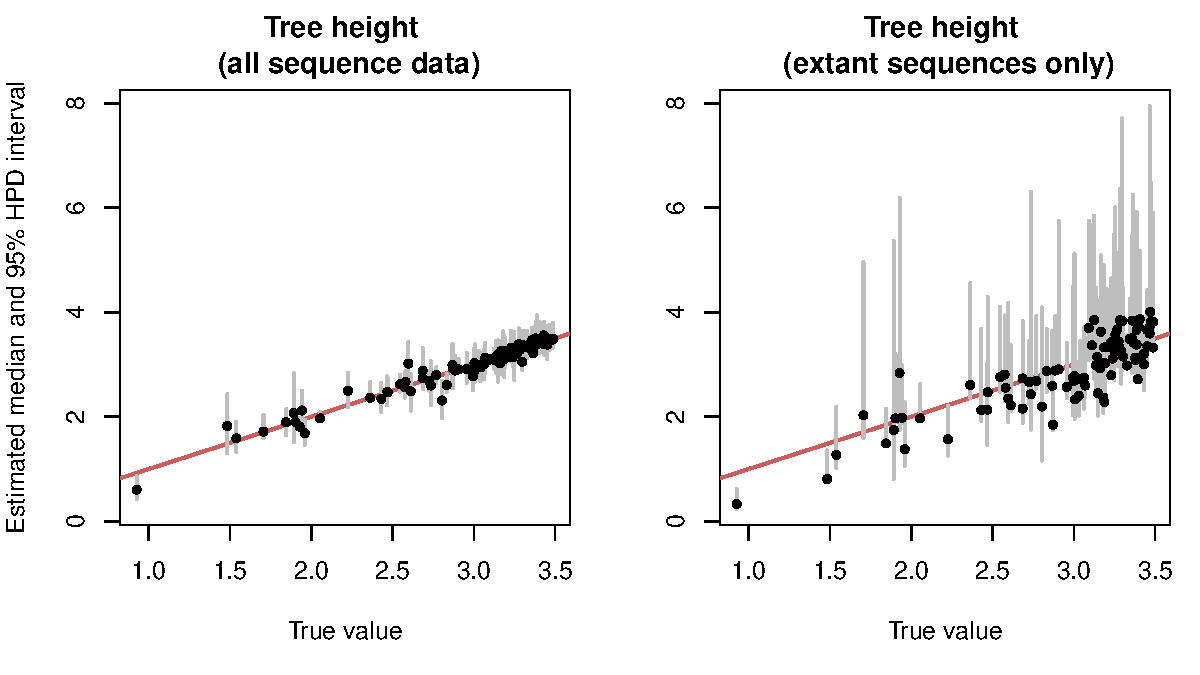
\includegraphics[width=\textwidth]{pics/Height_SA/Rplots.pdf}
\end{figure}

\end{frame}



%%%%%%%%%%%%%%%%%%%%%%%%%%%%%%%%%%%%%%%%%%%%%%


\begin{frame}{Comparative data of fossil tips vs only occurrence dates}

\setlength{\oddsidemargin}{0.1in} % adjust as necessary

\begin{columns}[c]

\begin{column}{.7\textwidth}
\begin{center}
\begin{figure}
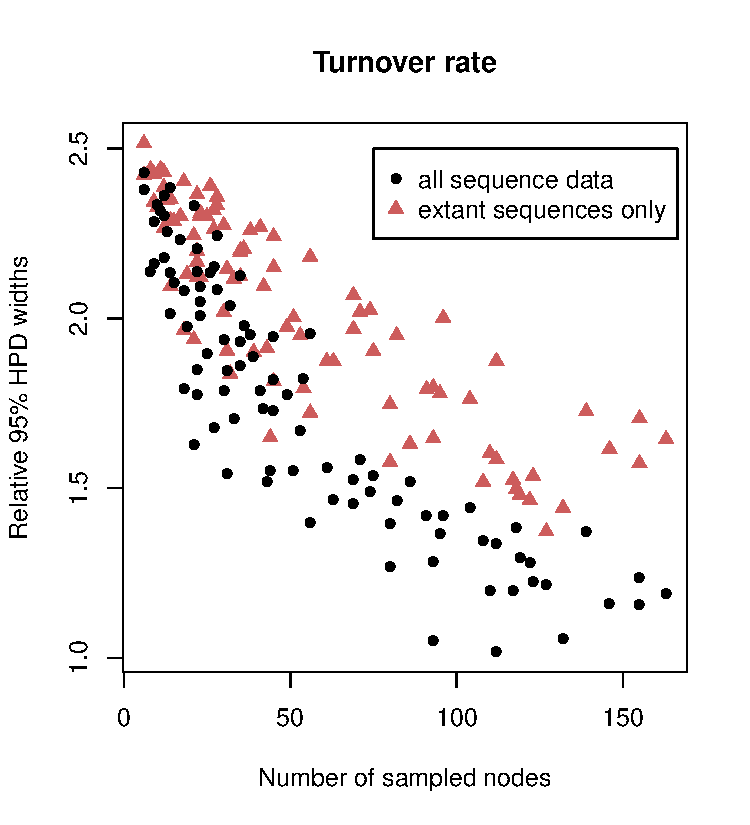
\includegraphics[height=0.65\textheight]{pics/TurnoverHPD/Rplots.pdf}
\end{figure}
\end{center}
 \end{column}
 
\begin{column}{.3\textwidth}
\begin{center}
turnover~rate~=~$\frac \mu \lambda$ 
\end{center}
 \end{column}    
\end{columns}

\end{frame}


%%%%%%%%%%%%%%%%%%%%%%%%%%%%%%%%%%%%%%%%%%%%%%


\begin{frame}{Biased estimates when not modelling sampled ancestors}

\begin{figure}
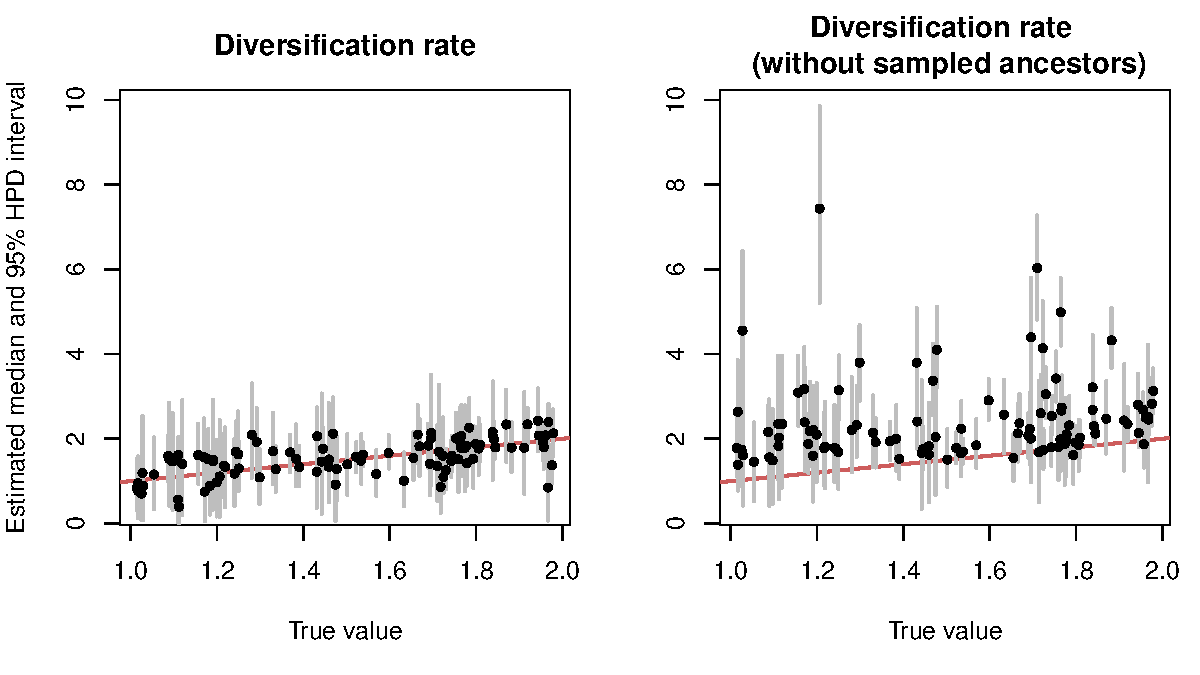
\includegraphics[width=\textwidth]{pics/SAvsNoSA/Rplots.pdf}
\end{figure}

\begin{center}
diversification rate = $\lambda-\mu$ 
\end{center}

\end{frame}